\section{Relationale Datenbanksprachen}
\label{sec:sql}

\textbf{Aggregatfunktionen}
\begin{items}
	\item Prinzip: Berechnung eines Werts aus Werten eines Attributs
	\item \underline{Join (natural)}: Kartesisches Produkt zweier Relationen
	\item Weitere in Standard SQL: count(), sum(), min(), max(), avg()
\end{items}

\textbf{SQL-Kern}
\begin{items}
	\item \underline{select} \\*
		Projektionsliste, \\*
		arithmetische Operationen und Aggregatfunktionen \\*
		\textbf{select distinct}: keine Dopplungen 
	\item \underline{from} \\*
		zu verwendende Relationen, ggf. Umbenennungen
	\item \underline{where} \\*
		Selektions- und Verbundbedingungen \\*
		geschachtelte Anfragen (wieder SFW-Block) \\*
	\item \underline{group by} \\*
		Gruppierung für Aggregatfunktionen
	\item \underline{having} \\*
		Selektionsbedingungen an Gruppen
\end{items}

\textbf{Self-Join}
\begin{items}
	\item Kartesisches Produkt einer Tabelle mit selbst
	\item Beispiel:
		\begin{lstlisting}[language=sql] 
select * from SNUser eins, SNUser zwei
	where eins.Alter < zwei.Alter
		\end{lstlisting}
		Vierspaltiges Ergebnis:
		\begin{lstlisting}[language=sql]
eins.Name, eins.Vorname,
zwei.Name, zwei.Vorname
		\end{lstlisting}
\end{items}

\textbf{Kartesisches Produkt}
\begin{items}
	\item Verbunde als explizite Operatoren:
		\begin{lstlisting}[language=sql]
select * from Kuenstler cross join Titel
		\end{lstlisting}
\end{items}

\textbf{Natürlicher Verbund}
\begin{items}
	\item Oft besser als herkömmliche Formulierung, weil
	\begin{enumeration}
		\item übersichtlicher
		\item weniger fehleranfällig (man vergisst leicht Attribut, wenn man alle aufzählen muss)
	\end{enumeration}
	\item
	\begin{lstlisting}[language=sql]
select * from Kuenstler natural join Titel
	\end{lstlisting}
\end{items}

\textbf{Theta-Join}
\begin{items}
	\item Verbund über Verbundsbedingungen
	\begin{lstlisting}[language=sql]
select * from Kuenstler 
	join Titel on Kuenstler.KID = Titel.KID
	\end{lstlisting}
	\item Beispiel: (AutoModell, AutoPreis), (BootModell, BootPreis) \\*
	Kunde will Boot und Auto, aber Boot soll billiger sein als Auto \\*
	\( \leadsto \text{Auto} \bowtie_{AutoPreis > BootPreis} \text{Boot} \)
\end{items}

\textbf{Outer, Left, Right Join}
\begin{figure}[H]\centering\label{SQLJoin}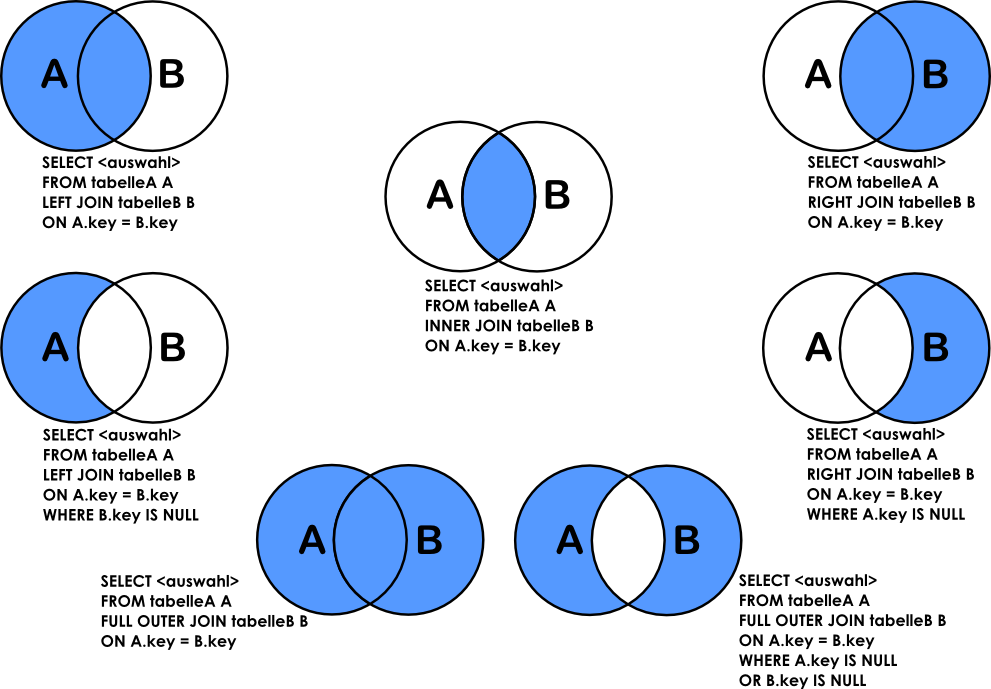
\includegraphics[width=0.4\textwidth]{SQLJoin}\end{figure}

\newpage

\textbf{where}
\begin{items}
	\item Trivial: \lstinline[language=sql]{where Buecher.Titel = "Titel"}
	\item Verbundbedingung (alternativ):
	\begin{lstlisting}[language=sql]
select Buecher.Titel, Buecher_Stichwort.Stichwort
	from Buecher, Buecher_Stichwort
	where Buecher.ISBN = Buecher_Stichwort.ISBN
	\end{lstlisting}
	\item \lstinline[language=sql]{like}: Ungewissheitsselektion (RegEx) \\*
	\lstinline[language=sql]{where attribut like spezialkonstante}
	\item \lstinline[language=sql]{in}: \lstinline[language=sql]{where ISBN in (select ISBN from Empfiehlt)}
\end{items}

\textbf{Mengen -- Vereinigung}
\begin{items}
	\item 
	\begin{lstlisting}[language=sql]
select A, B, C from R1 union 
	select A, C, D from R2
	\end{lstlisting}
	\item \lstinline[language=sql]{union}: Duplikate werden eliminiert
	\item \lstinline[language=sql]{union all}: Duplikate werden behalten
\end{items}

\textbf{Mengen -- Differenz}
\begin{items}
	\item Alle Mitarbeiter, die keine Studierenden sind:
	\begin{lstlisting}[language=sql]
select PANr from Mitarbeiter
	EXCEPT select PANr from Studenten
	\end{lstlisting}
\end{items}

\textbf{Mengen -- Durchschnitt}
\begin{items}
	\item Alle Mitarbeiter, die auch Studenten sind:
	\begin{lstlisting}[language=sql]
select PANr from Mitarbeiter
	INTERSECT select PANr from Studenten
	\end{lstlisting}
\end{items}

\textbf{Umbenennung}
\begin{items}
	\item
	\begin{lstlisting}[language=sql]
select ISBN, Preis * 1.44 as DollarPreis 
	from BuchVersionen
	\end{lstlisting}
\end{items}

\textbf{Grouping}
\begin{figure}[H]\centering\label{Zulassungen}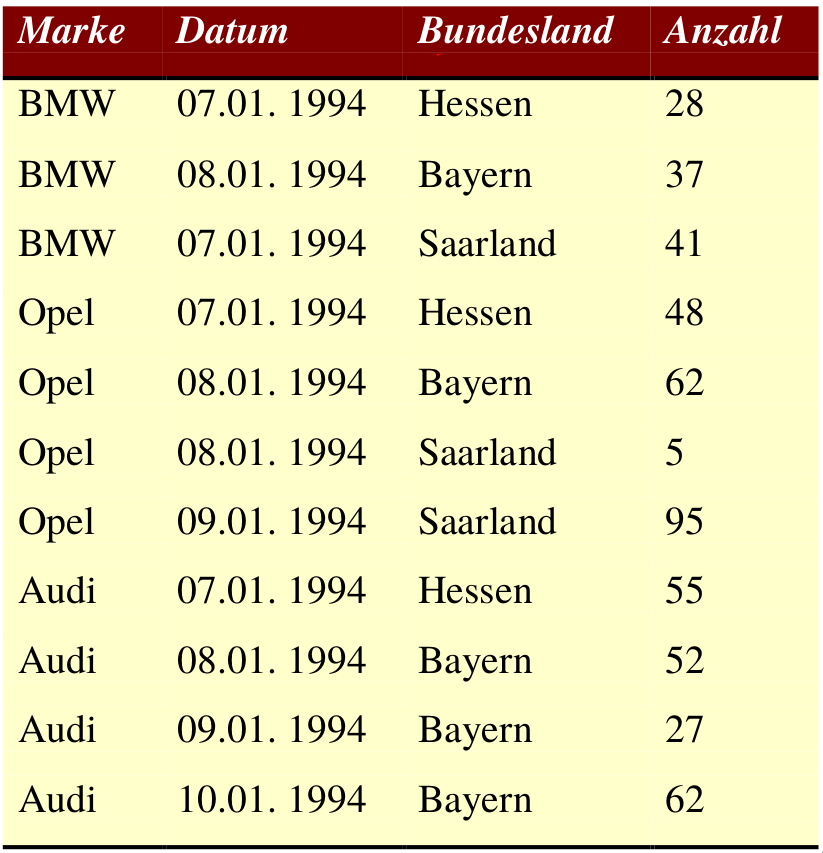
\includegraphics[width=0.2\textwidth]{Zulassungen}\end{figure}
\begin{items}
	\item
	\begin{lstlisting}[language=sql]
select Marke, sum(Anzahl)
	from Zulassungen
	group by Marke
	\end{lstlisting}
	\item 
	\begin{lstlisting}[language=sql]
select Marke, max(Anzahl)
	from Zulassungen
	group by Marke
	\end{lstlisting}
	\item \lstinline[language=sql]{having}-Bedingung:
	\begin{lstlisting}[language=sql]
select PANr, sum(Entlohnung)
	from anstellungen
	group by PANr
	having sum(entlohnung) > 10000
	\end{lstlisting}
\end{items}

\textbf{Quantoren}
\begin{items}
	\item \lstinline[language=sql]{any/some}:
	\begin{lstlisting}[language=sql]
select PANr, ImmaDatum
	from Studenten
	where MatNr = any (select MatNr from Prueft)
	\end{lstlisting}
	\item \lstinline[language=sql]{all}:
	\begin{lstlisting}[language=sql]
select Name from Kunde, Bestellung
	where Kunde.id = Bestellung.KundeID
	and bestellwert > ALL (SELECT avg(bestellwert) 
		from Bestellung group by KundeID)
	\end{lstlisting}
\end{items}

\newpage

\textbf{Sortieren}
\begin{items}
	\item \lstinline[language=sql]{order by}-Klausel:
	\begin{lstlisting}[language=sql]
select MatNr, Note from Prueft
	where V_Bez = 'DBS'
	order by Note asc
	\end{lstlisting}
	\item alternativ: \lstinline[language=sql]{desc}
\end{items}

\textbf{Nullwerte}
\begin{items}
	\item Vergleiche mit Nullwert: \lstinline[language=sql]{unknown} statt \lstinline[language=sql]{true} oder \lstinline[language=sql]{false} \\*
	\( \leadsto A=A \) keine Tautologie!
\end{items}

\textbf{Update}
\begin{items}
	\item
	\begin{lstlisting}[language=sql]
update relation set attribut1 = wert, ... 
	[where bedingung]
	\end{lstlisting}
\end{items}

\textbf{Delete}
\begin{items}
	\item
	\begin{lstlisting}[language=sql]
delete from relation [where bedingung]
	\end{lstlisting}
\end{items}

\textbf{Insert}
\begin{items}
	\item
	\begin{lstlisting}[language=sql]
insert into Kuenstler(KID, NAME, LAND, JAHR)
	values (1022, 'Raul Seixas', 
		1945, 'Brasilien')
	\end{lstlisting}
\end{items}

\begin{fragen}
	\begin{enumeration}
		\item Formulieren diverser (komplexer) SQL-Anfragen
		\item Vorgegebene geschachtelte Anfrage als nicht-geschachtelte schreiben
		\item Welche Join-Varianten kennen Sie?
		\item Geben Sie ein Beispiel an, in dem ein Self-Join sinnvoll ist.
		\item Was ist der Zusammenhang zwischen Vereinigung und Outer Join?
		\item Was ist eine Umbenennung im SQL-Kontext? Wann wird sie gebraucht?
		\item Geben Sie ein sinnvolles Beispiel für eine Anfrage an, die eine having-Klausel hat.
		\item Geben Sie ein Bespiel für eine Anfrage mit einer having-Klausel an, bei der man
		\begin{enumeration}
			\item die Klausel durch eine where-Klausel ersetzen kann,
			\item das nicht kann.
		\end{enumeration}
		\item Erläutern Sie, warum im SQL-Kontext ``A==A'' keine Tautologie ist.
	\end{enumeration}
\end{fragen}